\chapter{Lima}
\section*{5 juin 2015}
De Cusco a Lima, trajet en bus de luxe avec repas, films et sieges confortables on se croirait en avion. \newline
 \newline
\centerline{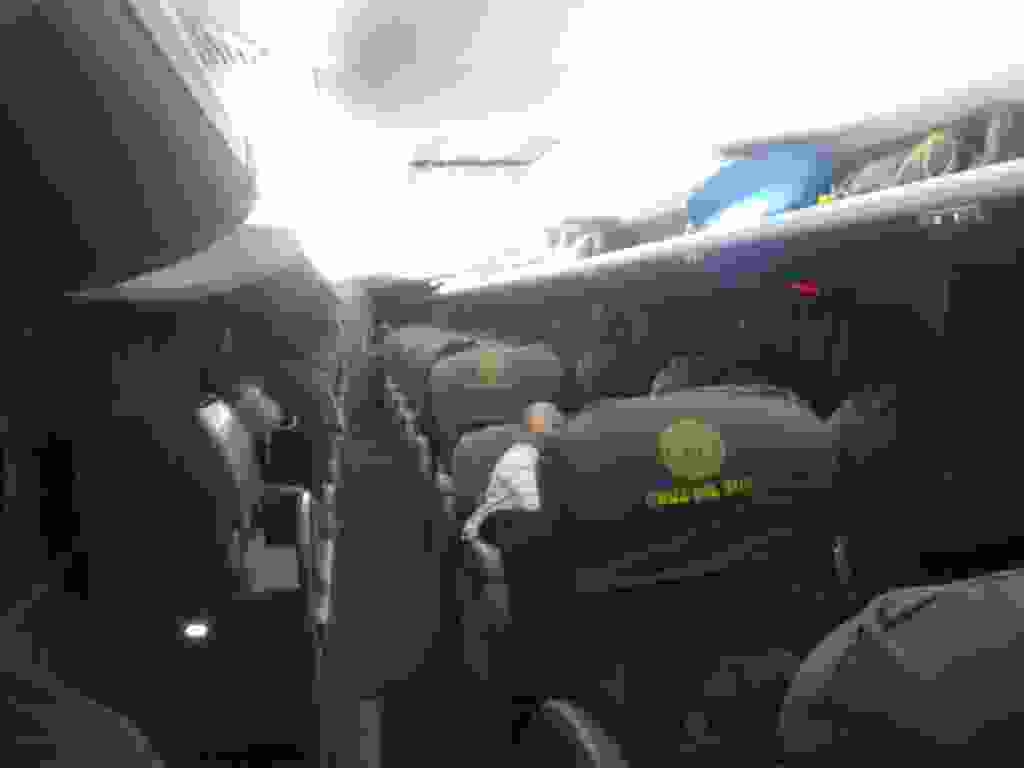
\includegraphics[width=\mywidth]{../wp-content/uploads/2015/06/P5304567-1024x768.jpg} } 
 \newline
 J´ai visité Lima en vélo : la ville est immense et le trafic énorme mais heureusement il y a quelques belles pistes cyclables sur les grandes avenues. \newline
 \newline
\centerline{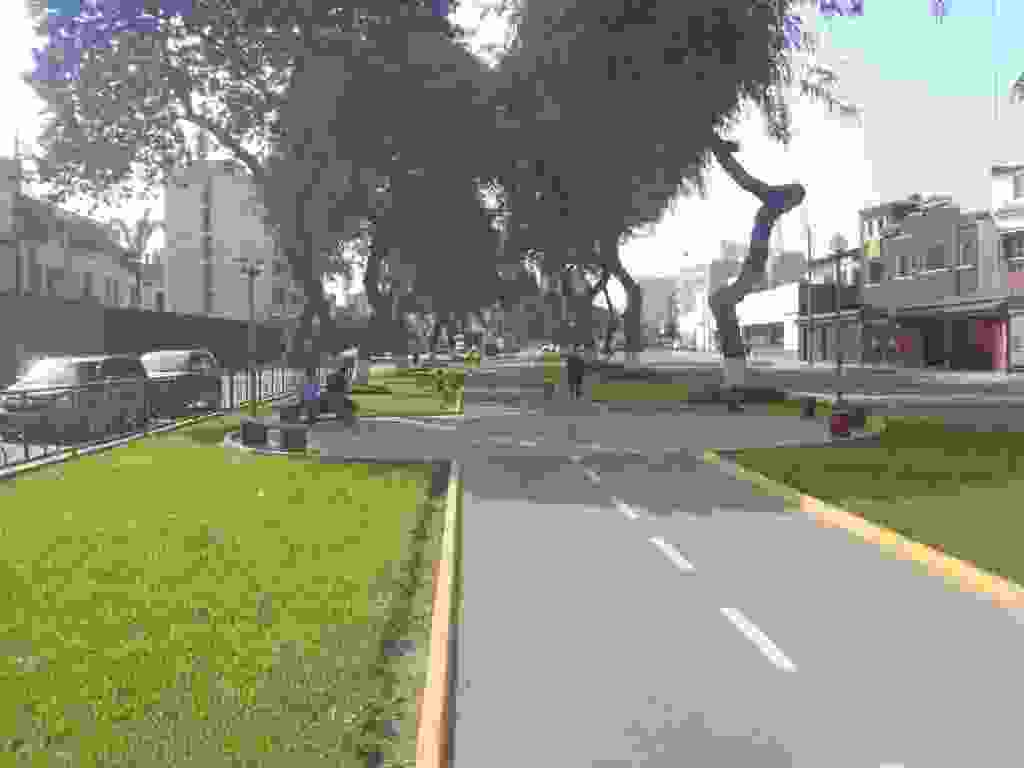
\includegraphics[width=\mywidth]{../wp-content/uploads/2015/06/P5314573-1024x768.jpg} } 
 \newline
 \newline
\centerline{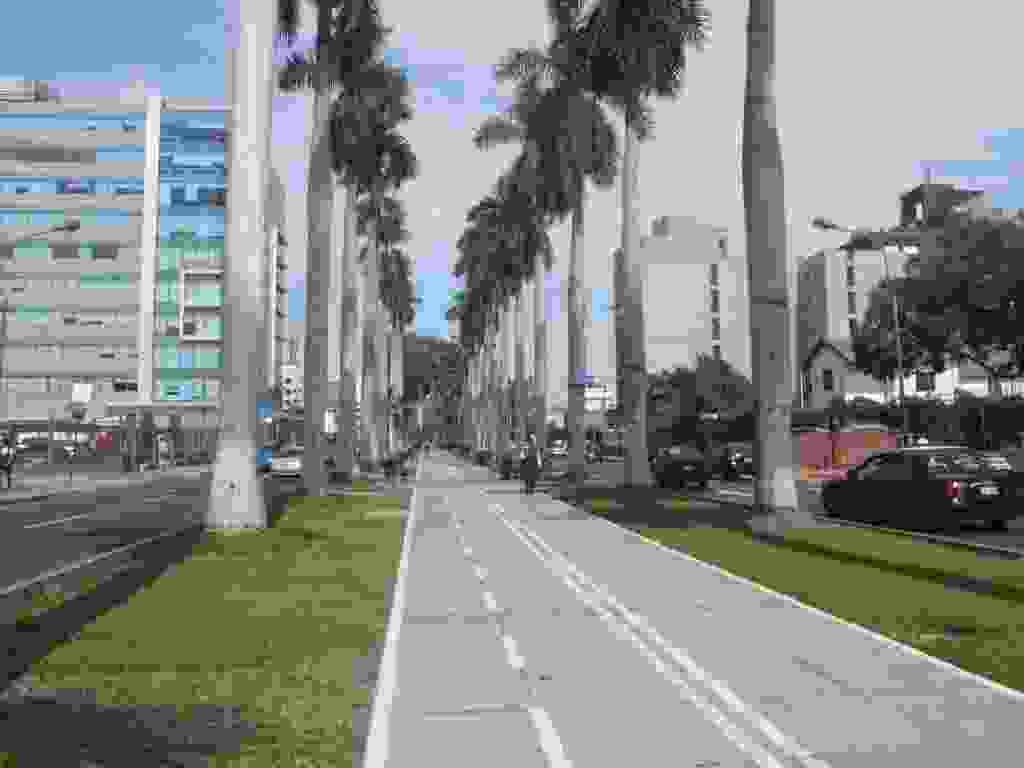
\includegraphics[width=\mywidth]{../wp-content/uploads/2015/06/P6014590-1024x768.jpg} } 
 \newline
 Le centre de Lima : \newline
 La Plaza San Martin \newline
 \newline
\centerline{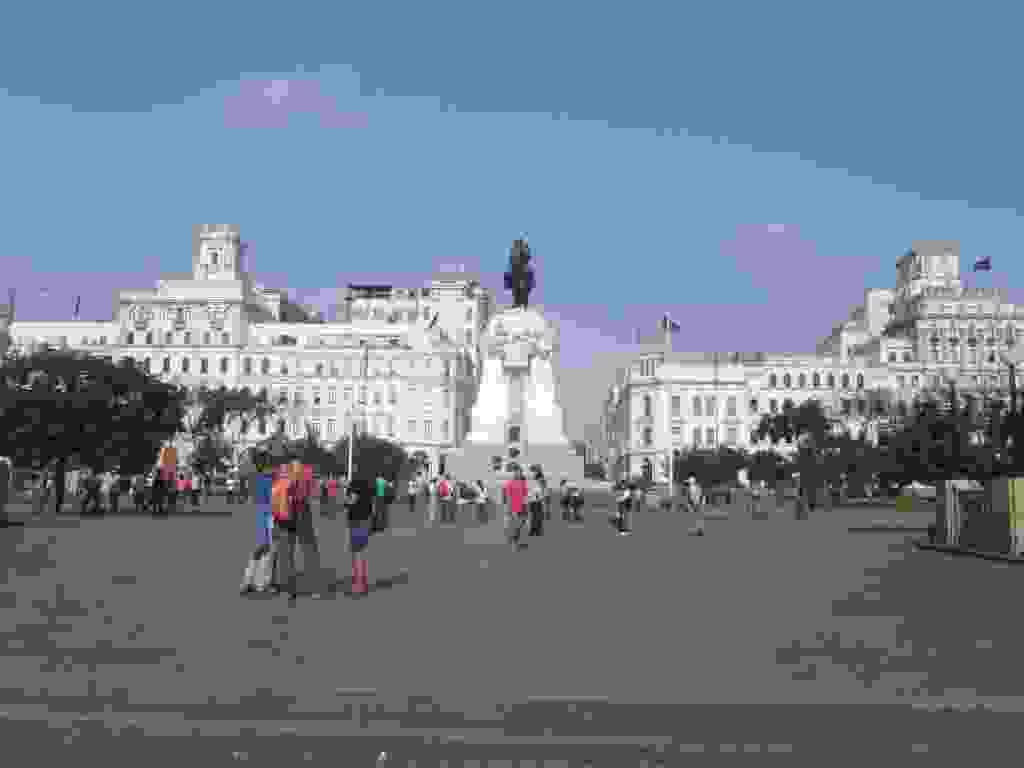
\includegraphics[width=\mywidth]{../wp-content/uploads/2015/06/P5314578-1024x768.jpg} } 
 \newline
 \newline
\centerline{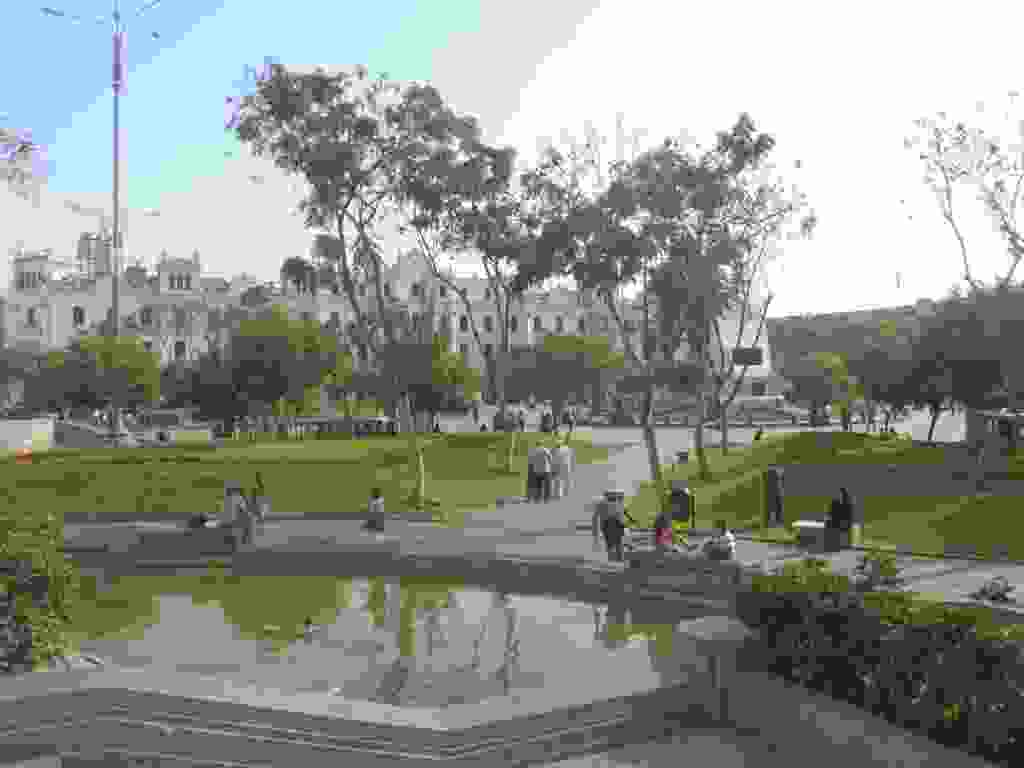
\includegraphics[width=\mywidth]{../wp-content/uploads/2015/06/P5314579-1024x768.jpg} } 
 \newline
 La Plaza de Armas avec la cathédrale et le palais gouvernemental \newline
 \newline
\centerline{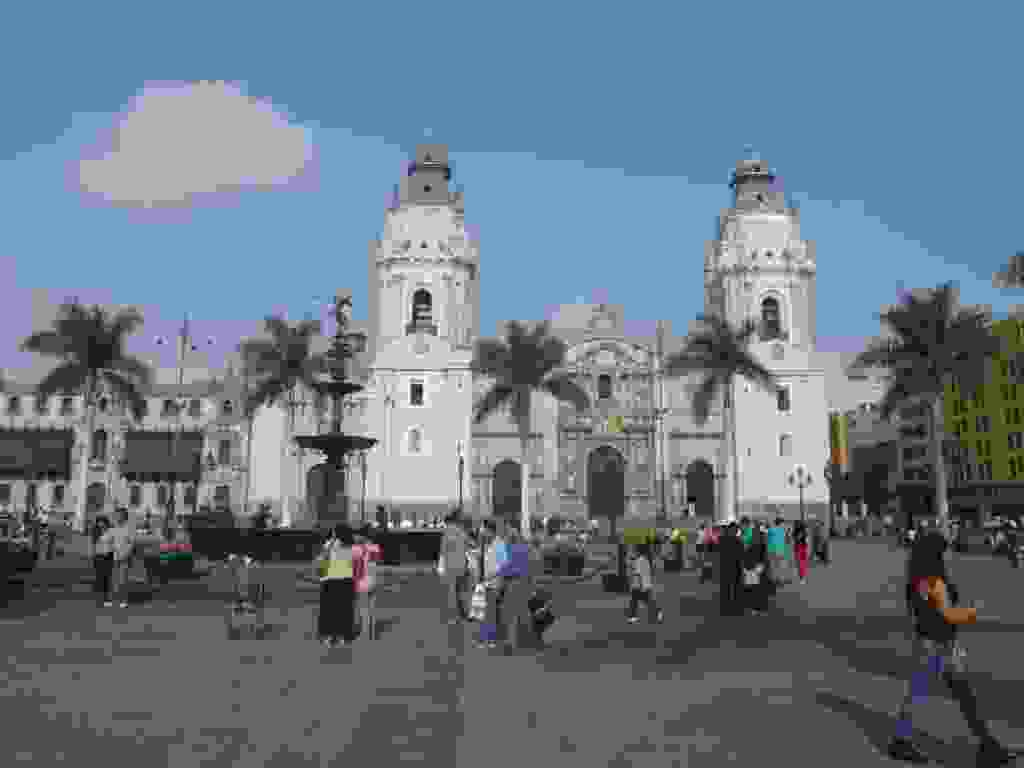
\includegraphics[width=\mywidth]{../wp-content/uploads/2015/06/P5314582-1024x768.jpg} } 
 \newline
 \newline
\centerline{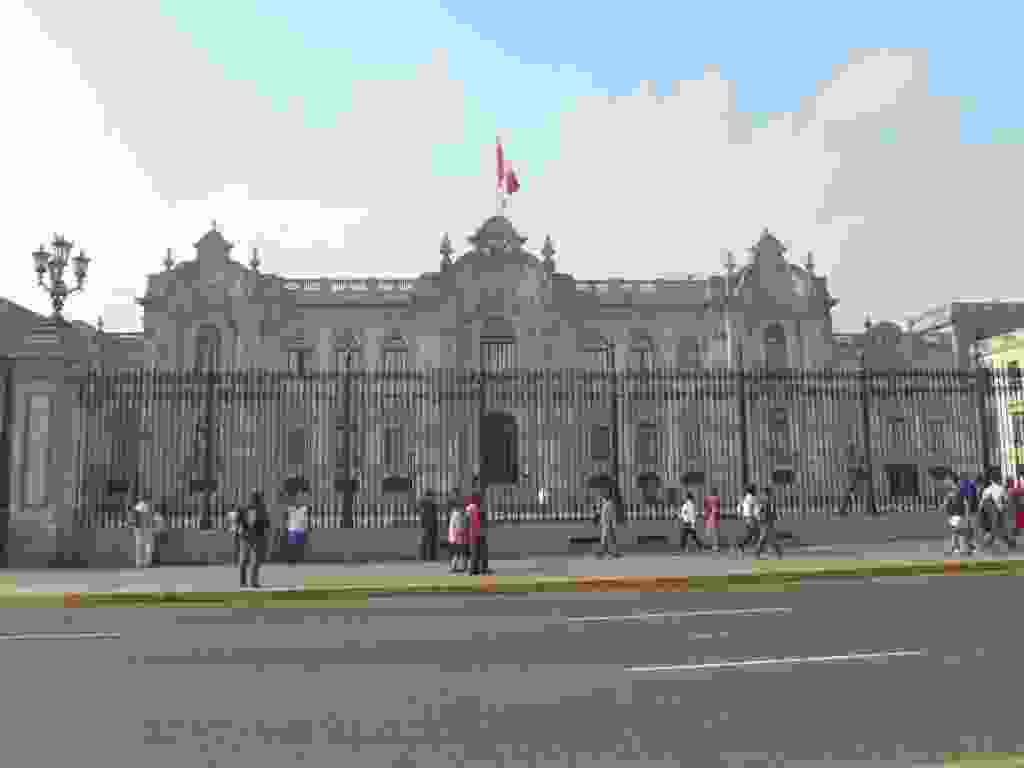
\includegraphics[width=\mywidth]{../wp-content/uploads/2015/06/P5314585-1024x768.jpg} } 
 \newline
 L´église San Francisco que j´ai visitée : avec notamment une belle bibliotheque et les catacombes oú des dizaines de milliers de personnes ont été enterrées. Dommage les photos étaient interdites a l´intérieur. \newline
 \newline
\centerline{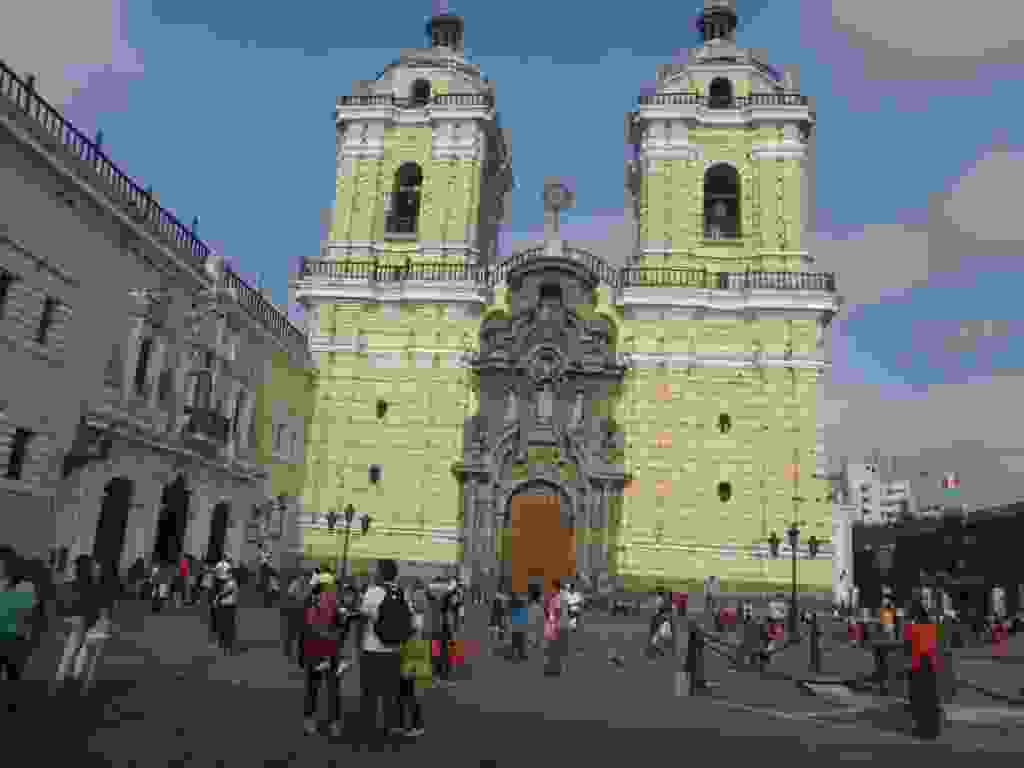
\includegraphics[width=\mywidth]{../wp-content/uploads/2015/06/P5314586-1024x768.jpg} } 
 \newline
 Le quartier Miraflores au sud de Lima : quartier touristique et aisé au bord de l´océan Pacifique. \newline
 \newline
\centerline{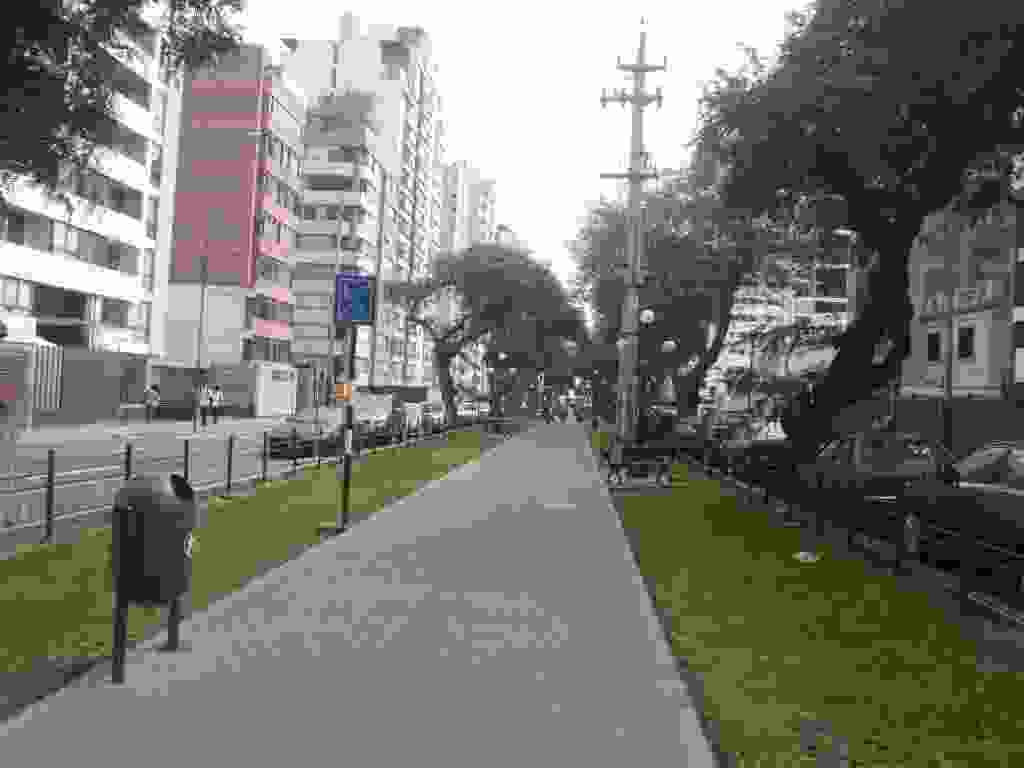
\includegraphics[width=\mywidth]{../wp-content/uploads/2015/06/P60145911-1024x768.jpg} } 
 \newline
 \newline
\centerline{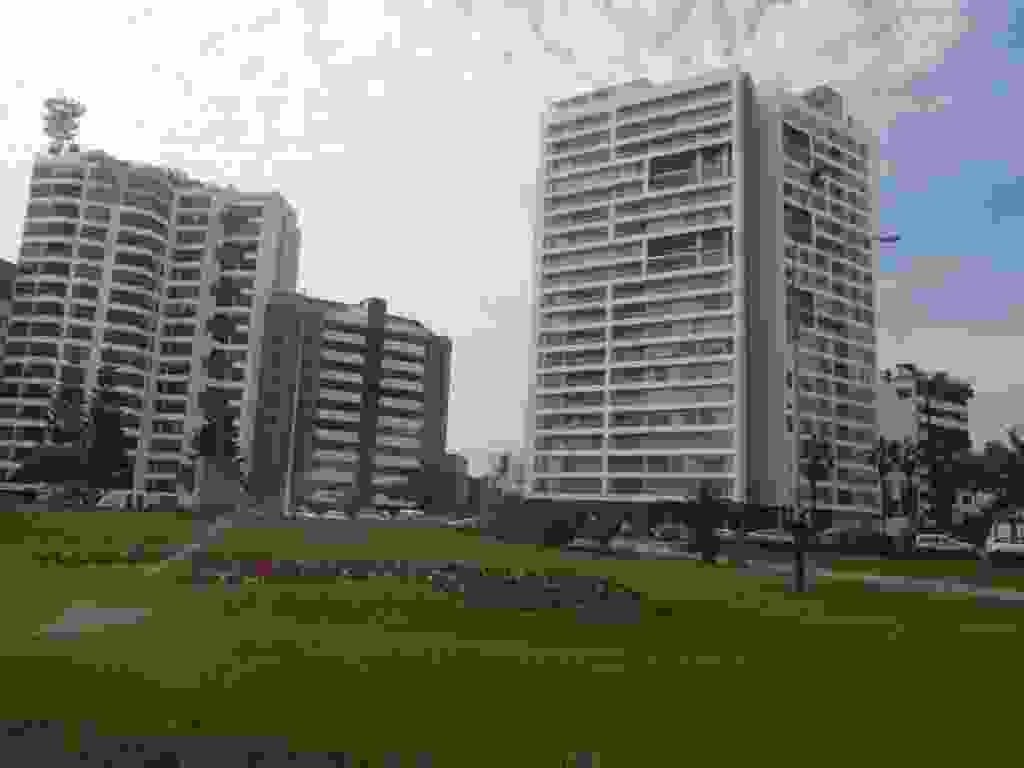
\includegraphics[width=\mywidth]{../wp-content/uploads/2015/06/P6014593-1024x768.jpg} } 
 \newline
 \newline
\centerline{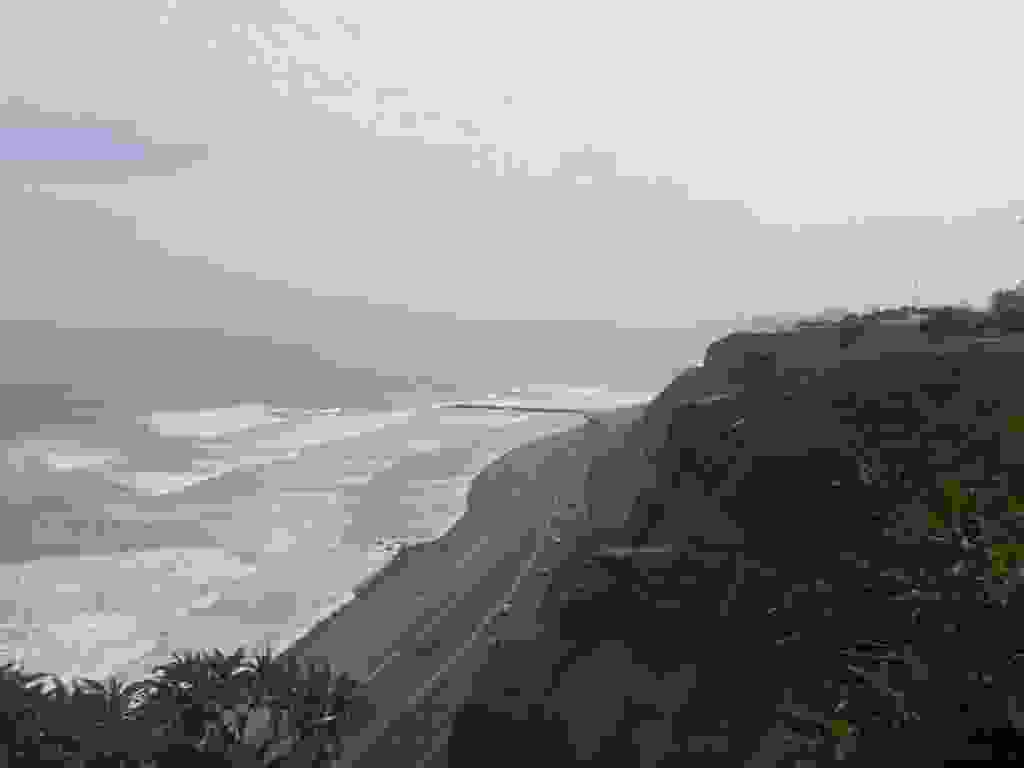
\includegraphics[width=\mywidth]{../wp-content/uploads/2015/06/P6014595-1024x768.jpg} } 
 \newline
 \newline
\centerline{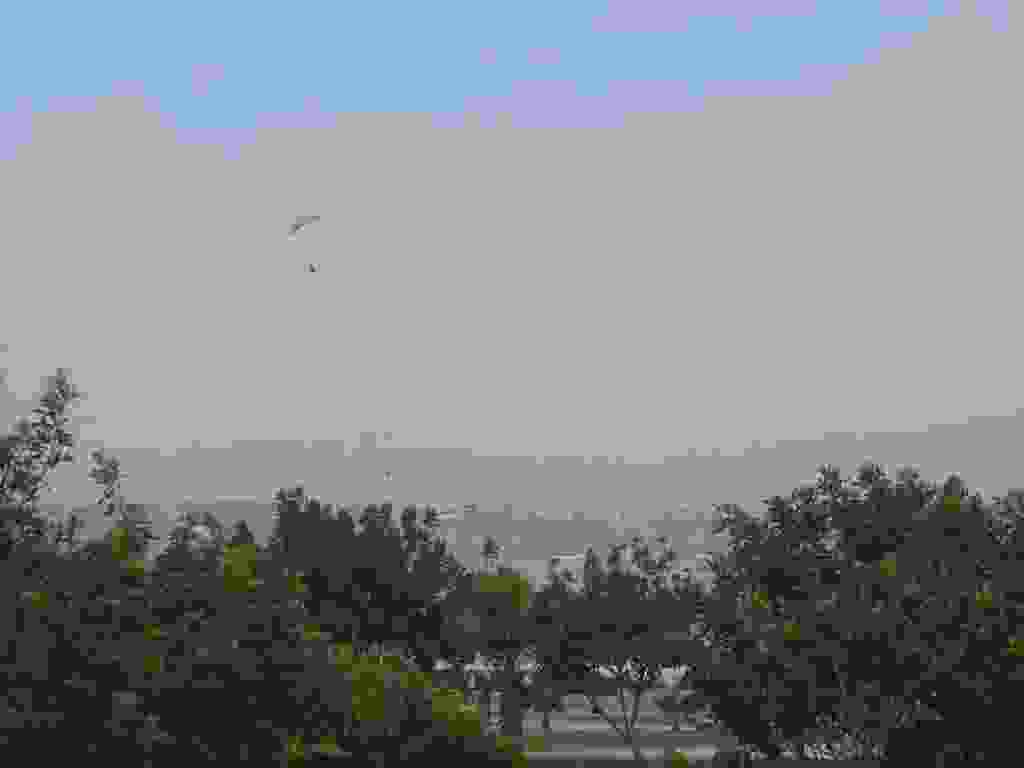
\includegraphics[width=\mywidth]{../wp-content/uploads/2015/06/P6014597-1024x768.jpg} } 
 \newline
 \newline
\centerline{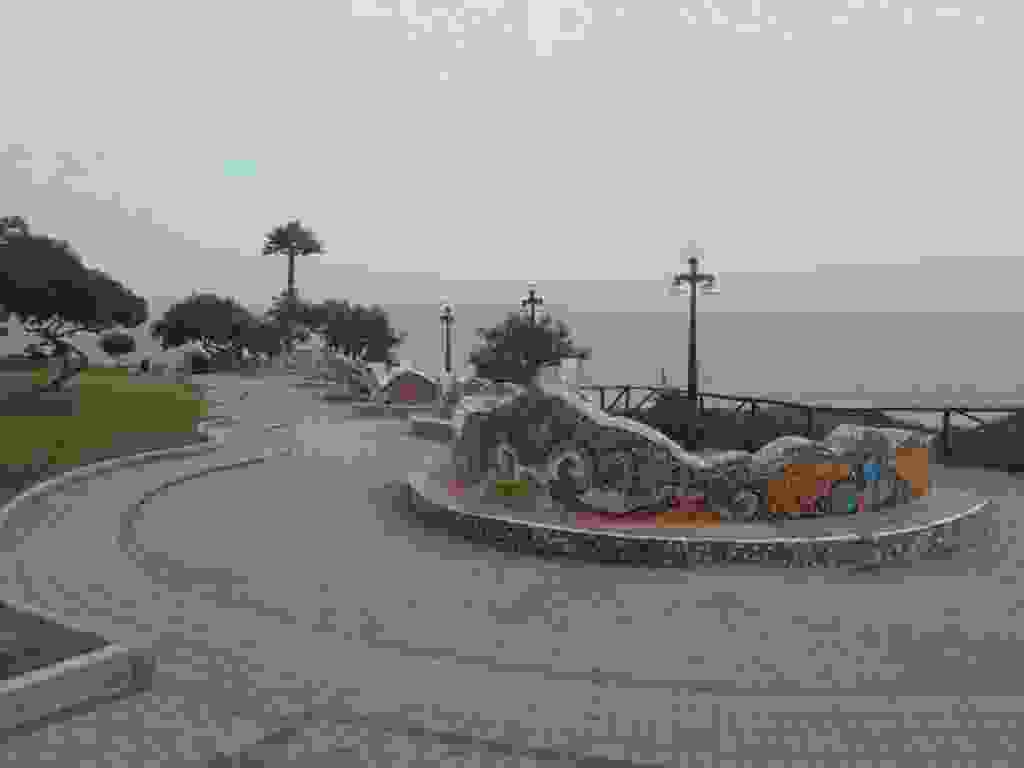
\includegraphics[width=\mywidth]{../wp-content/uploads/2015/06/P6014599-1024x768.jpg} } 
 \newline
 \newline
\centerline{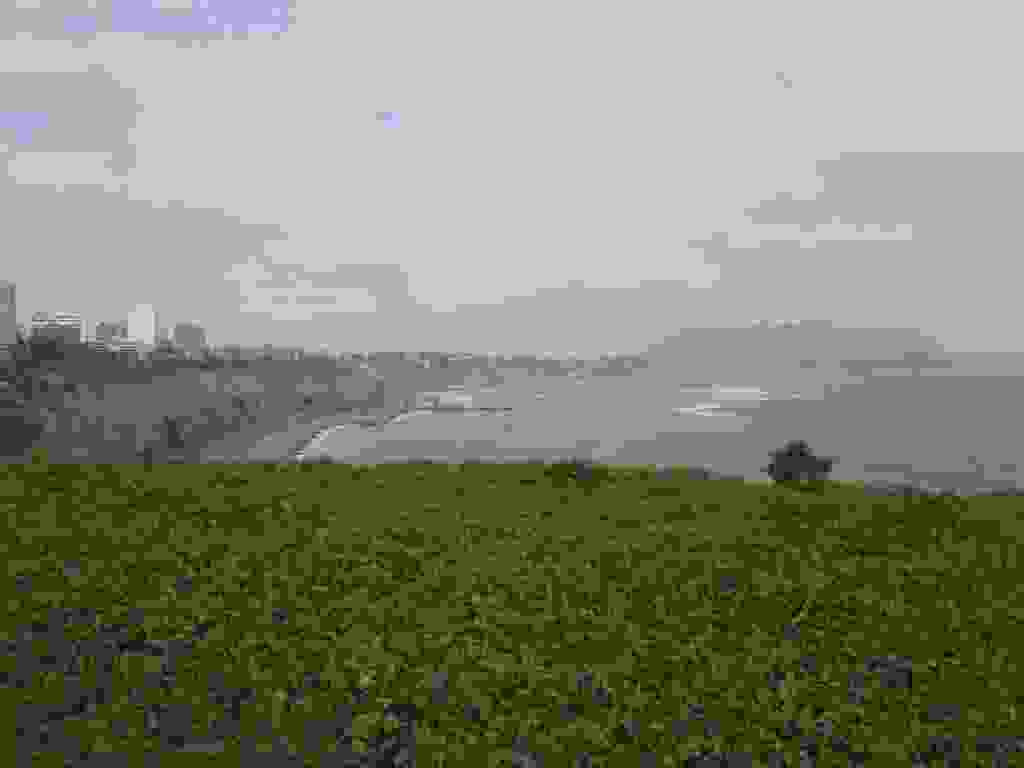
\includegraphics[width=\mywidth]{../wp-content/uploads/2015/06/P6014600-1024x768.jpg} } 
 \newline
 On y trouve de bons ceviches, «la» spécialité péruvienne de poisson et fruits de mer marinés. \newline
 \newline
\centerline{
\includegraphics[width=\mywidth]{../wp-content/uploads/2015/06/P6014602-1024x768.jpg} } 
 \newline
 Le quartier Barranco encore plus au sud : le quartier boheme de Lima. \newline
 \newline
\centerline{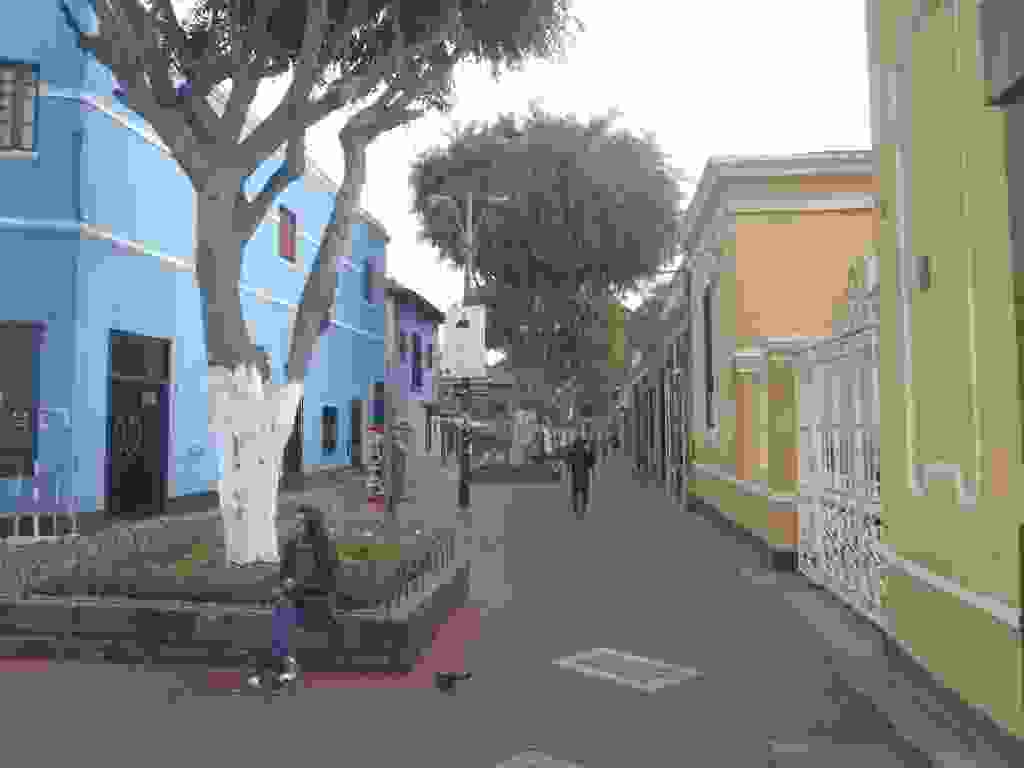
\includegraphics[width=\mywidth]{../wp-content/uploads/2015/06/P6014607-1024x768.jpg} } 
 \newline
 \newline
\centerline{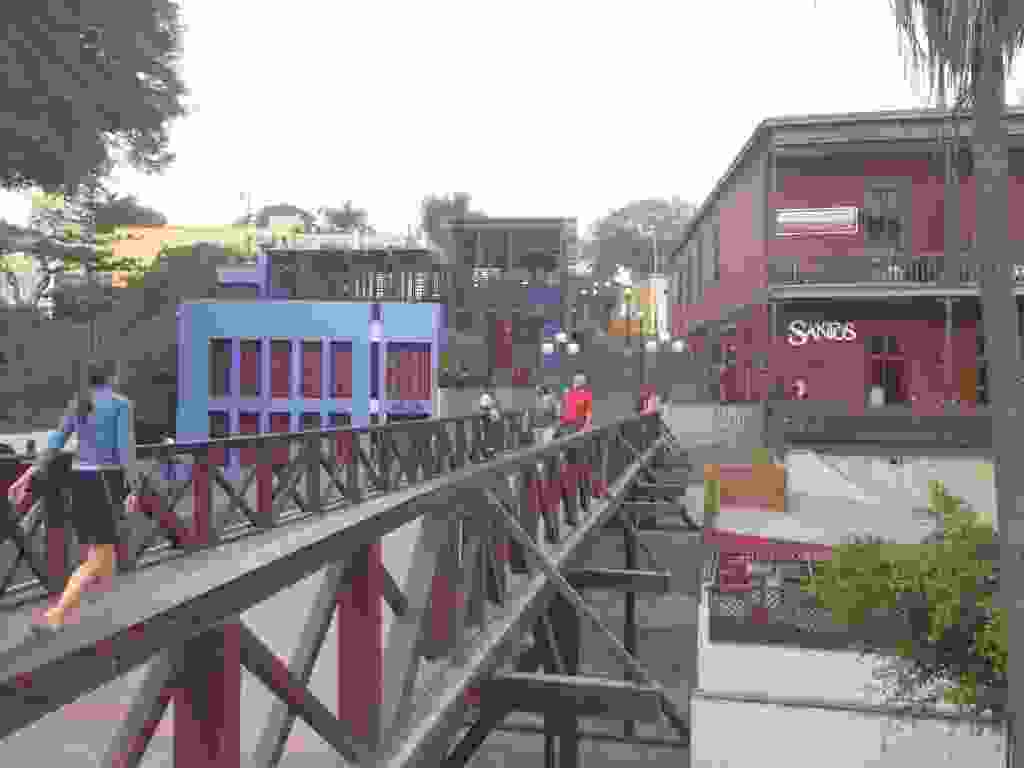
\includegraphics[width=\mywidth]{../wp-content/uploads/2015/06/P6014605-1024x768.jpg} } 
 \newline
 \newline
\centerline{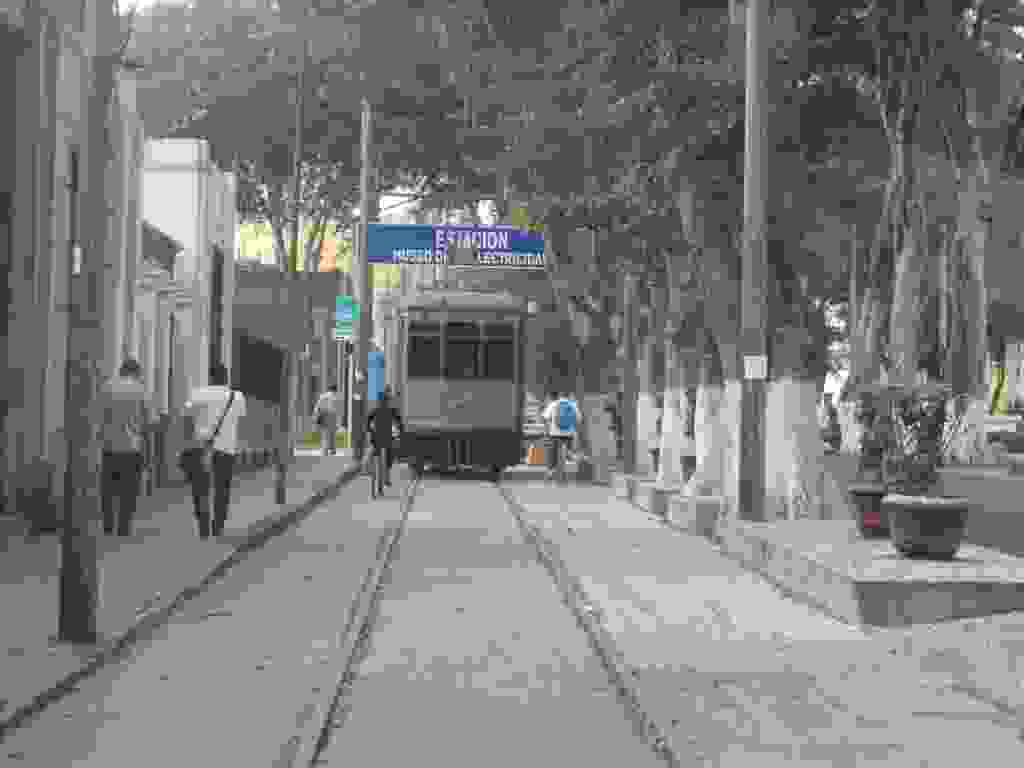
\includegraphics[width=\mywidth]{../wp-content/uploads/2015/06/P6014606-1024x768.jpg} } 
 \newline
 Enfin la petite pépite de Lima, le parc de la Reserva et son circuit des fontaines magiques : un parcours de 13 fontaines avec musique synchronisée aux jets d´eau. \newline
 \newline
\centerline{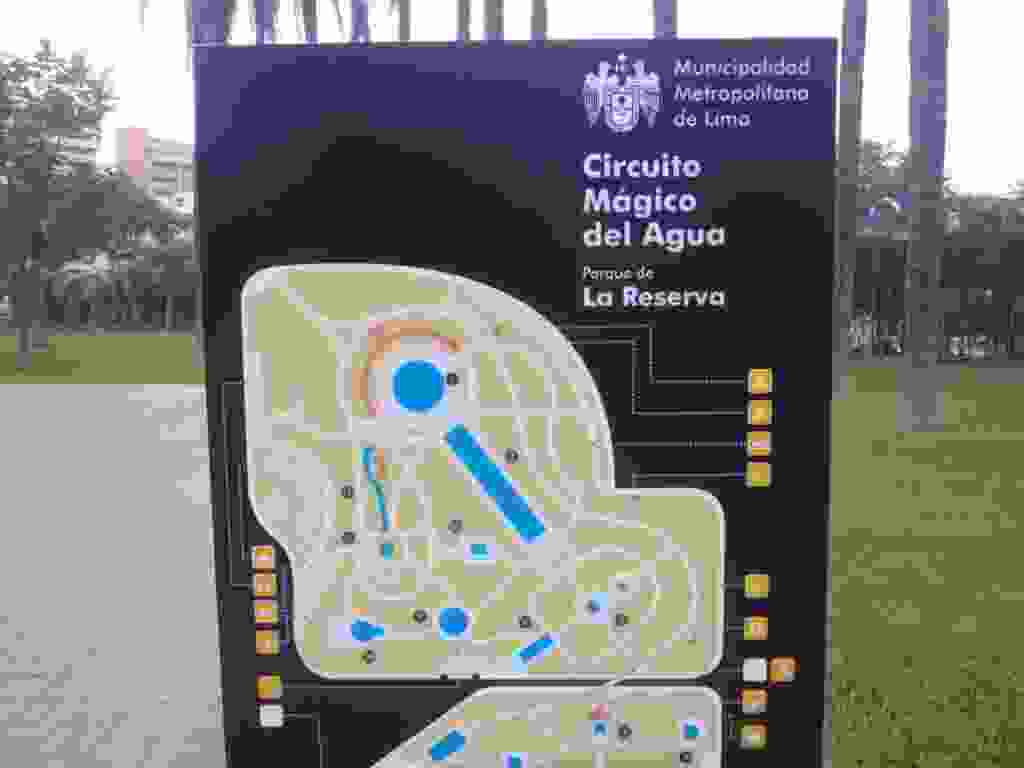
\includegraphics[width=\mywidth]{../wp-content/uploads/2015/06/P6024611-1024x768.jpg} } 
 \newline
 \newline
\centerline{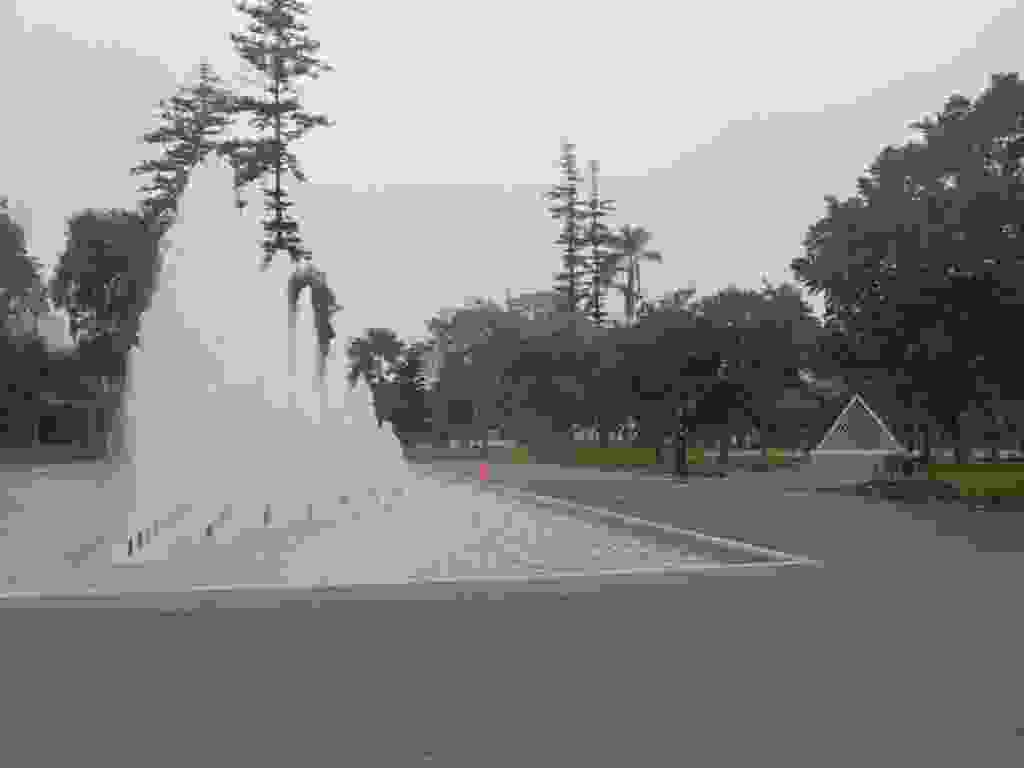
\includegraphics[width=\mywidth]{../wp-content/uploads/2015/06/P6024610-1024x768.jpg} } 
 \newline
 \newline
\centerline{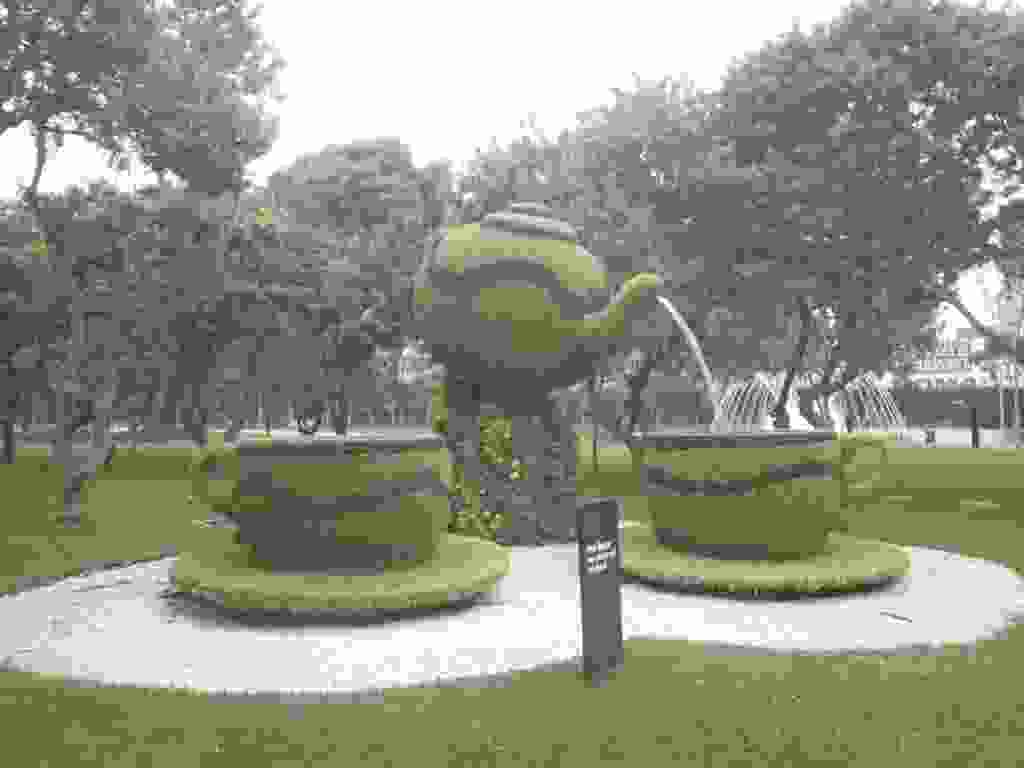
\includegraphics[width=\mywidth]{../wp-content/uploads/2015/06/P6024615-1024x768.jpg} } 
 \newline
 \newline
\centerline{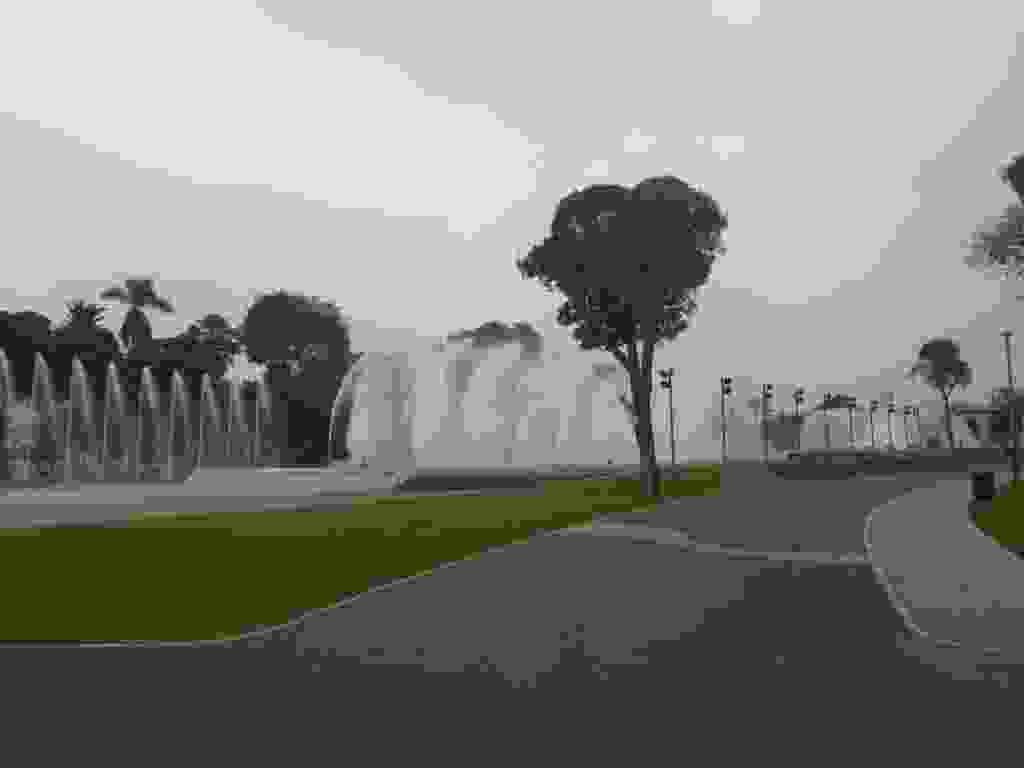
\includegraphics[width=\mywidth]{../wp-content/uploads/2015/06/P6024617-1024x768.jpg} } 
 \newline
 \newline
\centerline{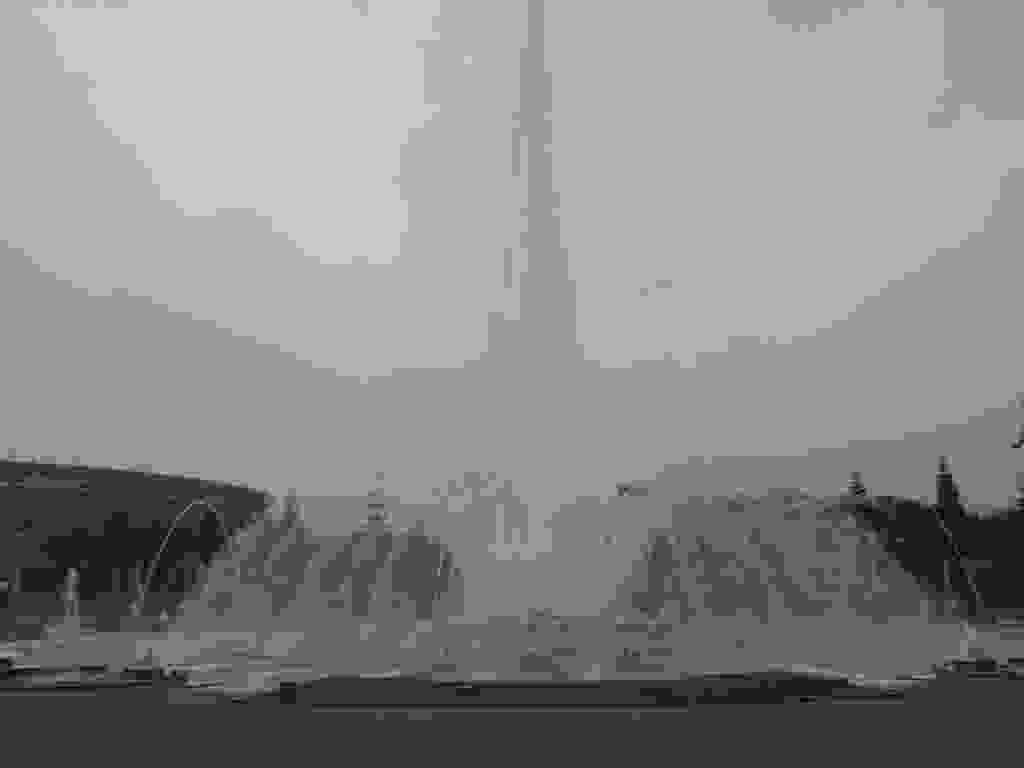
\includegraphics[width=\mywidth]{../wp-content/uploads/2015/06/P6024619-1024x768.jpg} } 
 \newline
 \newline
\centerline{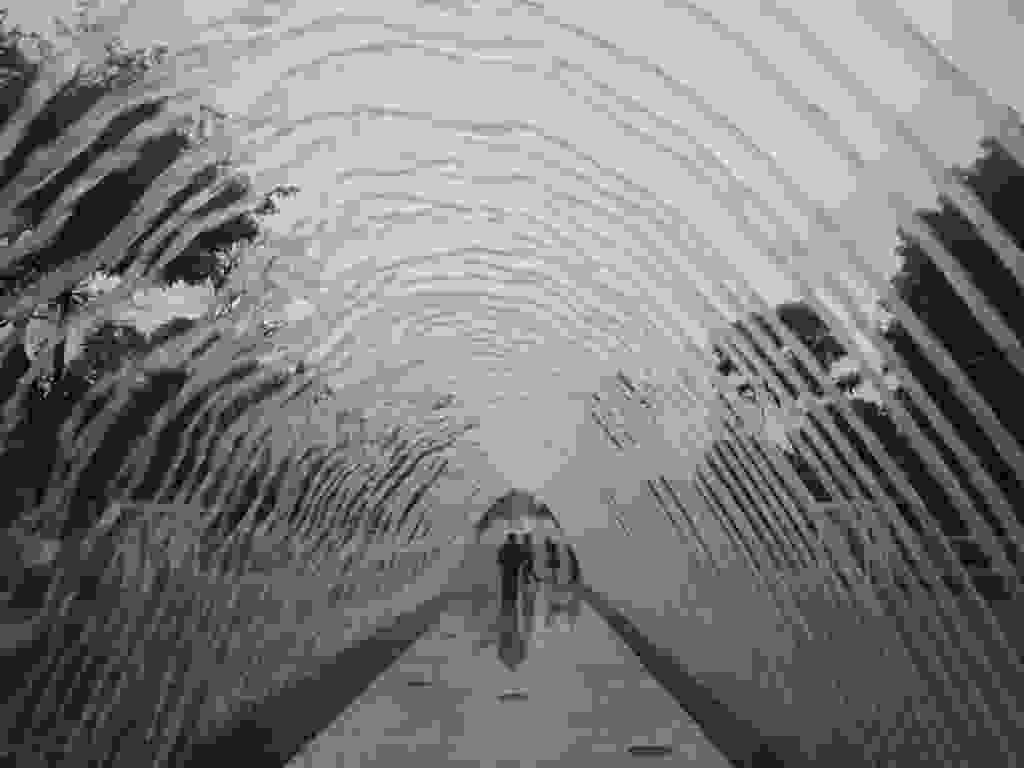
\includegraphics[width=\mywidth]{../wp-content/uploads/2015/06/P6034631-1024x768.jpg} } 
 \newline

\newpage
 
